\subsection{Multilevel coarse grid corrections and a multigrid method}
\Label{sc:mg-fd}
To describe a multigrid algorithm, we first need to have a multiple
level of grids, say $\mathcal T_\ell$ with $\ell=1:J$ and $\mathcal T_1=\mathcal T_h$ being the
finest mesh.  There are many ways to obtain multiple level of grids
and one simple definition of the grid points in $\mathcal T_\ell$ is as follows:
$$
        x_i^\ell=\frac{i}{2^{J+1-\ell}},\quad i=1,2,\cdots, N_\ell, \ell=1,2,\cdots,J,
$$
where $N_\ell=2^{J+1-\ell}-1$.  Note that $\mathcal T_{\ell-1}$ can be viewed as being obtained
by adding midpoints of the subintervals in ${\mathcal T}_{\ell}$.  For each $\ell$
the set of above nodes will be denoted by $\mathcal N_\ell$.

\begin{figure}[!htb]
\begin{center}
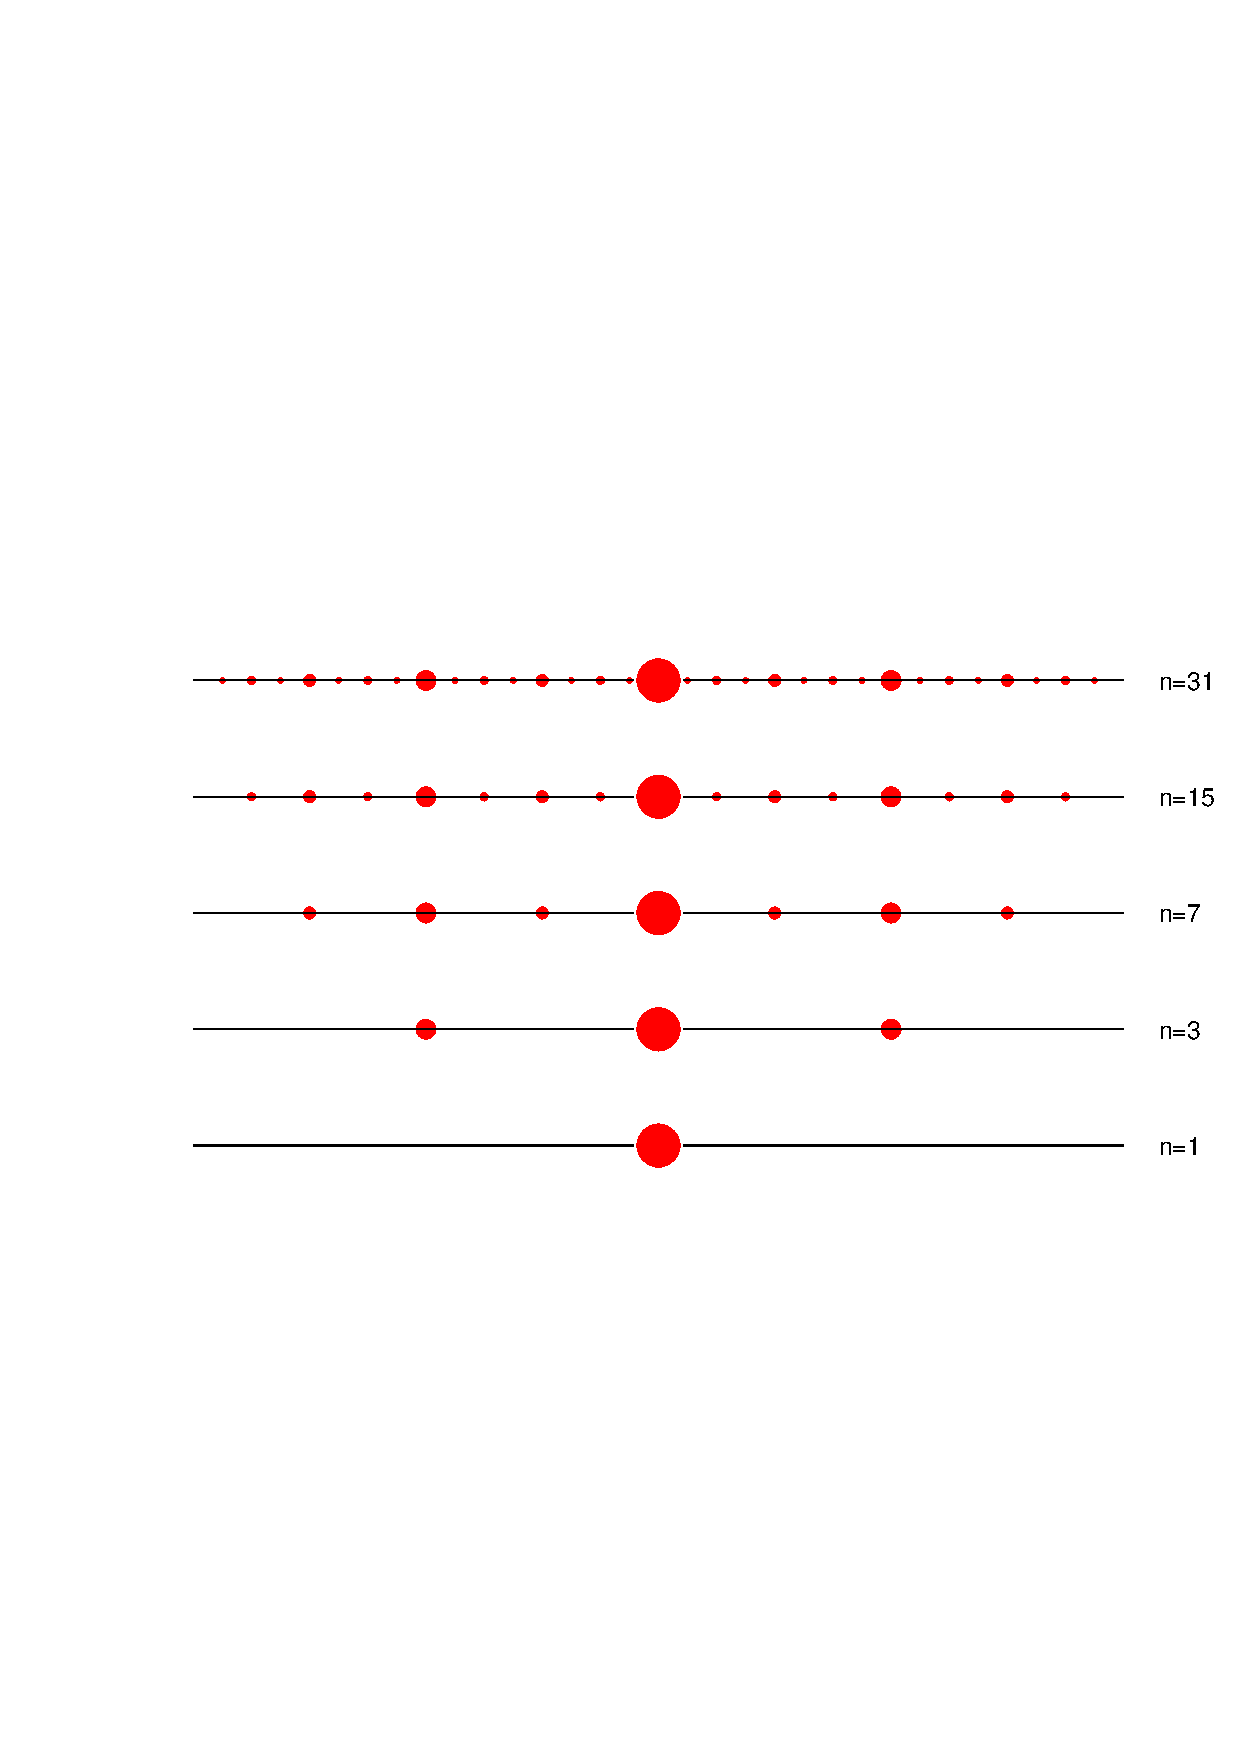
\includegraphics[width=3in]{pictures/manygr.pdf}
\end{center}
\caption{Multiple grids in one dimension
\label{fig:manygrids}}
\end{figure}


With our previous experiences in two-grid method, the description of a
multigrid method is not very difficult.  In fact, the multiple level
grids are treated by treating each two consecutive grids, say $\mathcal T_{\ell-1}$
versus $\mathcal T_{\ell}$.  If we think $\mathcal T_{\ell-1}$ versus $\mathcal T_{\ell}$ like
$\mathcal T_h$ and $\mathcal T_{2h}$, then there is not much new in the multigrid
setting.


Let us give some on details the definition of the restriction and
prolongation matrices.  The restriction matrix $R_{\ell-1}^\ell: R^{N_{\ell-1}}
\mapsto R^{N_{\ell}}$ can be defined by
\begin{equation}\Label{restrictk}
\gamma^{\ell}=R_{\ell-1}^\ell\gamma^{\ell-1}: \;
\gamma^{\ell}_i={1\over2}\gamma^{\ell-1}_{2i-1}+\gamma^{\ell-1}_{2i}+{1\over2}\gamma^{\ell-1}_{2i+1}.
\end{equation}
In matrix form 
\begin{equation}
\label{1drestriction}
R_{\ell-1}^\ell=\left(
\begin{array}{ccccccccc}
\frac{1}{2}& 1&\frac{1}{2}&&&&&&\\
&&\frac{1}{2}&1&\frac{1}{2}&&&&\\
&&&&\frac{1}{2}&1&\frac{1}{2}&&\\
&&&&&&\ddots&&\\
&&&&&&\frac{1}{2}&1&\frac{1}{2}\\
\end{array}
\right)
\end{equation}
For a special case, when $N_1=7, N_2=3$, we have 
\begin{equation}
\label{1drestriction3}
R_1^2=\left(
\begin{array}{ccccccc}
\frac{1}{2}& 1&\frac{1}{2}&0&0&0&0\\
0&0&\frac{1}{2}&1&\frac{1}{2}&0&0\\
0&0&0&0&\frac{1}{2}&1&\frac{1}{2}\\
\end{array}
\right).
\end{equation}




The prolongation matrix
$P_{\ell}^{\ell-1}: R^{N_{\ell}}
\mapsto R^{N_{\ell-1}}$ can be defined as 
\begin{equation}\Label{prolongk}
~~\epsilon^{\ell-1}=P^{\ell-1}_{\ell}\epsilon^{\ell}: \; \epsilon^{\ell-1}_{2i}=\epsilon^{\ell}_i, \epsilon^{\ell-1}_{2i+1}
= {1\over~2}(\epsilon^{\ell}_i+\epsilon^{\ell}_{i+1}), \; i=1:N_{\ell}.
\end{equation}

With the restriction and prolongation matrices in hands, we can now
present a multilevel version of the earlier two-grid algorithm.  As
mentioned before, the idea is to repeat this two grid process for the
coarse grid by using an even coarser grid.  The resulting algorithm is
just a desired multigrid algorithm. 


Using the convolution with stride notation, the restriction subprocess can also be written as 
$R\ast_2: \mathbb R^{N_\ell}\rightarrow  \mathbb R^{N_{\ell+1}}$, for any $v\in \mathbb R^{N_\ell}, u=(R\ast_2 v)\in R^{N_{\ell+1}}$ with
$$
 (R\ast_2 v)_i=\frac 12 v_{2i-1} +v_{2i}+\frac 12 v_{2i+1},\quad  \mbox{namely}\quad R\ast_2v=R_{\ell-1}^\ell v
$$
where $R=[\frac 12,1,\frac12]$ and $R_{\ell-1}^\ell $ is defined by \eqref{1drestriction}.

Next 
let $u^{\ell+1}=\sum\limits_{j=1}^{n_{\ell+1}}\mu_{j}^{\ell+1}\phi^{\ell+1}_{j}
=(  \mu^{\ell+1}, \phi^{\ell+1})_{l^2}$, then we have
\begin{equation}
\begin{split}
u^{\ell+1}&=( \mu^{\ell+1}, \phi^{\ell+1})_{l^2}
=( \mu^{\ell+1}, R\ast_2\phi^{\ell})_{l^2}=(R\ast_2^{\top} \mu^{\ell+1}, \phi^{\ell})_{l^2}\\
&=\sum\limits_{j=1}^{n_{\ell}}\left(R\ast_2^{\top} \mu^{\ell+1}\right)_{j}\phi^{\ell}_{j}.
\end{split}
\end{equation}
The prolongation subprocess can be written as 
$R\ast_2^T: \mathbb R^{N_{\ell+1}}\rightarrow \mathbb R^{N_\ell}$, for any $v\in \mathbb R^{N_{\ell+1}}, u=(R\ast_2^T v)\in R^{N_\ell}$ with
$$
(R\ast_2^T v)_{2i}=v_i,\quad (R\ast_2^T v)_{2i+1}=\frac 12 (v_{i+1} +v_i),\quad  \mbox{namely}\quad R\ast_2^Tv=P^{\ell-1}_\ell v
$$
where $R=[\frac 12,1,\frac12]$.

Using the convolution notation, the subprocess to apply $A_\ell$ to 
a vector $v\in \mathbb R^{N_\ell}$ can be written as
$A_\ell\ast: \mathbb R^{N_\ell}\rightarrow \mathbb R^{N_\ell}$, for any $v\in \mathbb R^{N_\ell}, r=(A_\ell\ast v)\in R^{N_\ell}$ with
$$
(A_\ell\ast v)_{i}=\frac{1}{h_\ell}( -v_{i-1}+2v_i-v_{i+1})
$$
where $A_\ell=\frac{1}{h_\ell}[-1,2,-1]$.

\newpage

\begin{breakablealgorithm}%[!htb]
	\caption{A multigrid algorithm $\mu = {\text{MG1}}(b; \mu^0; J,\nu_1, \cdots, \nu_J)$}
\label{alg:L-Slash11dm}
\begin{algorithmic}
%	 \State 
%		$$
%		u \leftarrow u^0.
%		$$
	\State Set up
		$$
		b^1 = b, \quad \mu^{1}=\mu^0. 
		$$
		\State Smoothing and restriction from fine to coarse level (nested)
		\For{$\ell = 1:J$}
		\For{$i = 1:\nu_\ell$}
		\State
		\begin{equation}\label{eq:smoothing}
		\mu^{\ell} \leftarrow \mu^{\ell} + S^\ell \ast (b^\ell - A_\ell \ast \mu^{\ell}).
		\end{equation}
		\EndFor
		\State Form restricted residual and set initial guess:
		$$
		\mu^{\ell+1} \leftarrow 0, \quad b^{\ell+1} \leftarrow R \ast_2 (b^\ell -  A_\ell \ast \mu^{\ell}), A_{\ell+1} = R       \ast_2 A_\ell \ast (R\ast_2^\top).
		$$
		\EndFor
		\State Prolongation and restriction from coarse to fine level
		\For{$\ell = J-1:1$}
		\State
		$$
		\mu^{\ell} \leftarrow \mu^{\ell} + R  \ast_2^{\top} \mu^{\ell+1}.
		$$
%		%		\IF{V-cycle}
%		\For{$i = 1:\nu_\ell$}
%		\State
%		$$
%		u^{\ell,i} \leftarrow u^{\ell,i-1} + [B^{\ell,i}]^T (f^\ell - A^{\ell} u^{\ell,i-1})
%		$$
%		\EndFor
%		%		\ENDIF
		\EndFor
		\State
		$$
		\mu \leftarrow \mu^{1}.
		$$
	\end{algorithmic}
\end{breakablealgorithm}


Application of Multigrid:
		Given $\mu^{(0)}$, for $m=1,2,\cdots$ till convergence
		$$
		\mu^{(m)}= {\text{MG1}}(b; \mu^{{(m-1)}}; J,\nu_1, \cdots, \nu_J).
		$$
		
\example Let $f(x)=1$. Consider 
\begin{equation}\label{1Dposi}
\left\{
\begin{aligned}
-u''&= f, \,\, 0<x<1, \\
 u(0)&=u(1)=0.
\end{aligned}
\right.
\end{equation}
The true solution $u=\frac12 x(1-x)$. Given the partition with the grid points 
$x_i=\frac{i}{n+1}, i=0,1,\cdots,n+1$, then by finite element discretization, 
we obtain 
\begin{equation}\label{matrix}
A\ast \mu =b, A=\frac{1}{h}[-1,2,-1].
\end{equation}
Use gradient descent method and multigrid to solve \eqref{matrix} with random initial guess $\mu^0$.



\begin{figure}[!ht]
\centering
\setlength{\abovecaptionskip}{0pt}
\setlength{\belowcaptionskip}{0pt}
\includegraphics[width=8.3cm]{figures/mgcompare.png}
\caption{Comparison GD with Multigrid}
\label{fig:Hmesh}
\end{figure}





